\documentclass[a4paper, amsfonts, amssymb, amsmath, reprint, showkeys, nofootinbib, twoside]{revtex4-1}
\usepackage[english]{babel}
\usepackage[utf8]{inputenc}
\usepackage[colorinlistoftodos, color=green!40, prependcaption]{todonotes}
\usepackage[pdftex, pdftitle={Article}, pdfauthor={Author}]{hyperref}
\usepackage{amsthm}
\usepackage{mathtools}
\usepackage{physics}
\usepackage{xcolor}
\usepackage{caption}
\usepackage{hyperref}
%\hypersetup{colorlinks=true, linkcolor=blue, urlcolor = blue}
\usepackage{amsmath}
\usepackage{amssymb}
\usepackage{graphicx}
\graphicspath{Images}
\usepackage[left=23mm,right=13mm,top=35mm,columnsep=15pt]{geometry} 
\usepackage{adjustbox}
\usepackage{placeins}
\usepackage[T1]{fontenc}
\usepackage{float}
%\usepackage{longtable}
\usepackage{csquotes}
\usepackage{refstyle}
\usepackage{lipsum}

\begin{document}

\title{Determination of Band Gap and Resistivity of Conductors and Semi-Conductors Using Four Probe}
\author{Swaroop Ramakant Avarsekar}
\email{swaroop.avarsekar@niser.ac.in}
\affiliation{School of Physical Sciences, National Institute of Science Education and Research, HBNI, Jatni -752050, India}
\date{\today}

	
\begin{abstract}
This experiment aims to determine the resistivity of Si, Al and Ge at room temperature and hence studying the resistivity as a function of temperature for the case of Ge and determine the band gap energy of Ge. The measurement of resistivity uses four probe method to overcome the contact resistance and accurately determine the resistivity. We found resistivity of Al as $(2.8\pm0.17)\times10^{-8}$ $\Omega m$, resistivity of Si as $0.370\pm0.008$ $\Omega m$, and resistivity of Ge as $(1.75\pm0.03)\times10^{-7}$ $\Omega m$ with the band gap of $0.70\pm0.06$ eV.
\end{abstract}
	
\keywords{Fermi level, Resistivity, Band-gap}
	
\maketitle

\section{Theory}
Four probe is a apparatus to determine the resistivity of the semi-conductors. The current is passed through outer two probes and the voltage is measured from the inner probes as shown in figure(\ref{1}). This method eliminates the contact resistance since the same probes are used to measure the resistance as provided with the current as well unlike the case of two probe with different resistance measuring probe and current source. This is used for accurate measurement of resistivity. 

The four probes are collinearly equally spaced made of Tungsten. It is assumed that resistivity of the sample is uniform, with flat surface and no surface leakage irrespective of material be a conductor or insulator. Measurements should be made which has high recombination rate surface. The resistivity for the large sample is given by:

\begin{equation}
	\rho_o=\frac{V}{I}2\pi S
\end{equation}  

where S is the distance between two probes, which is equal between the probes.

For resistivity of thin sheet samples for non conducting bottom surface where W is the width of the sample. Resistivity then becomes :

\begin{equation}
	\rho=\frac{\rho_o}{G_7(W/S)}
\end{equation}

For small values of W/S less than 0.25, ${G_7(W/S)}$ becomes:
\begin{equation}
	{G_7(W/S)}=\frac{2S}{W}log_e2
\end{equation}

For semi-conductors, temperature dependence of resistivity is governed by equation below:
  \begin{equation}
  	R=R_oe^{E_g/2KT}
  \end{equation}

Therefore, the equation to determine band gap is
\begin{equation}\label{w}
	E_g=2KTlog_e\rho
\end{equation}

\begin{figure}[H]
	\centering
	\includegraphics[width=6cm, height=7cm]{1}
	\caption{Working of four probe}
	\label{1}
\end{figure}

\section{Experiment}
Place the sample on the base plate of the four probe, with the apparatus placed in oven. Use constant current power supply for Ge and Al and low current power supply for Si. Note down the current and voltage readings by increasing the current at room temperature. We could see linear relationship as Ohms Law. To determine the band gap , we study the resistivity of Ge at various temperatures by keeping the current fixed and varying the temperature from $80^{\circ}$ C-$100^{\circ}$ C and noting down the voltage readings. Temperature is varied using PID controller with an oven.

\begin{figure}[H]
	\centering
	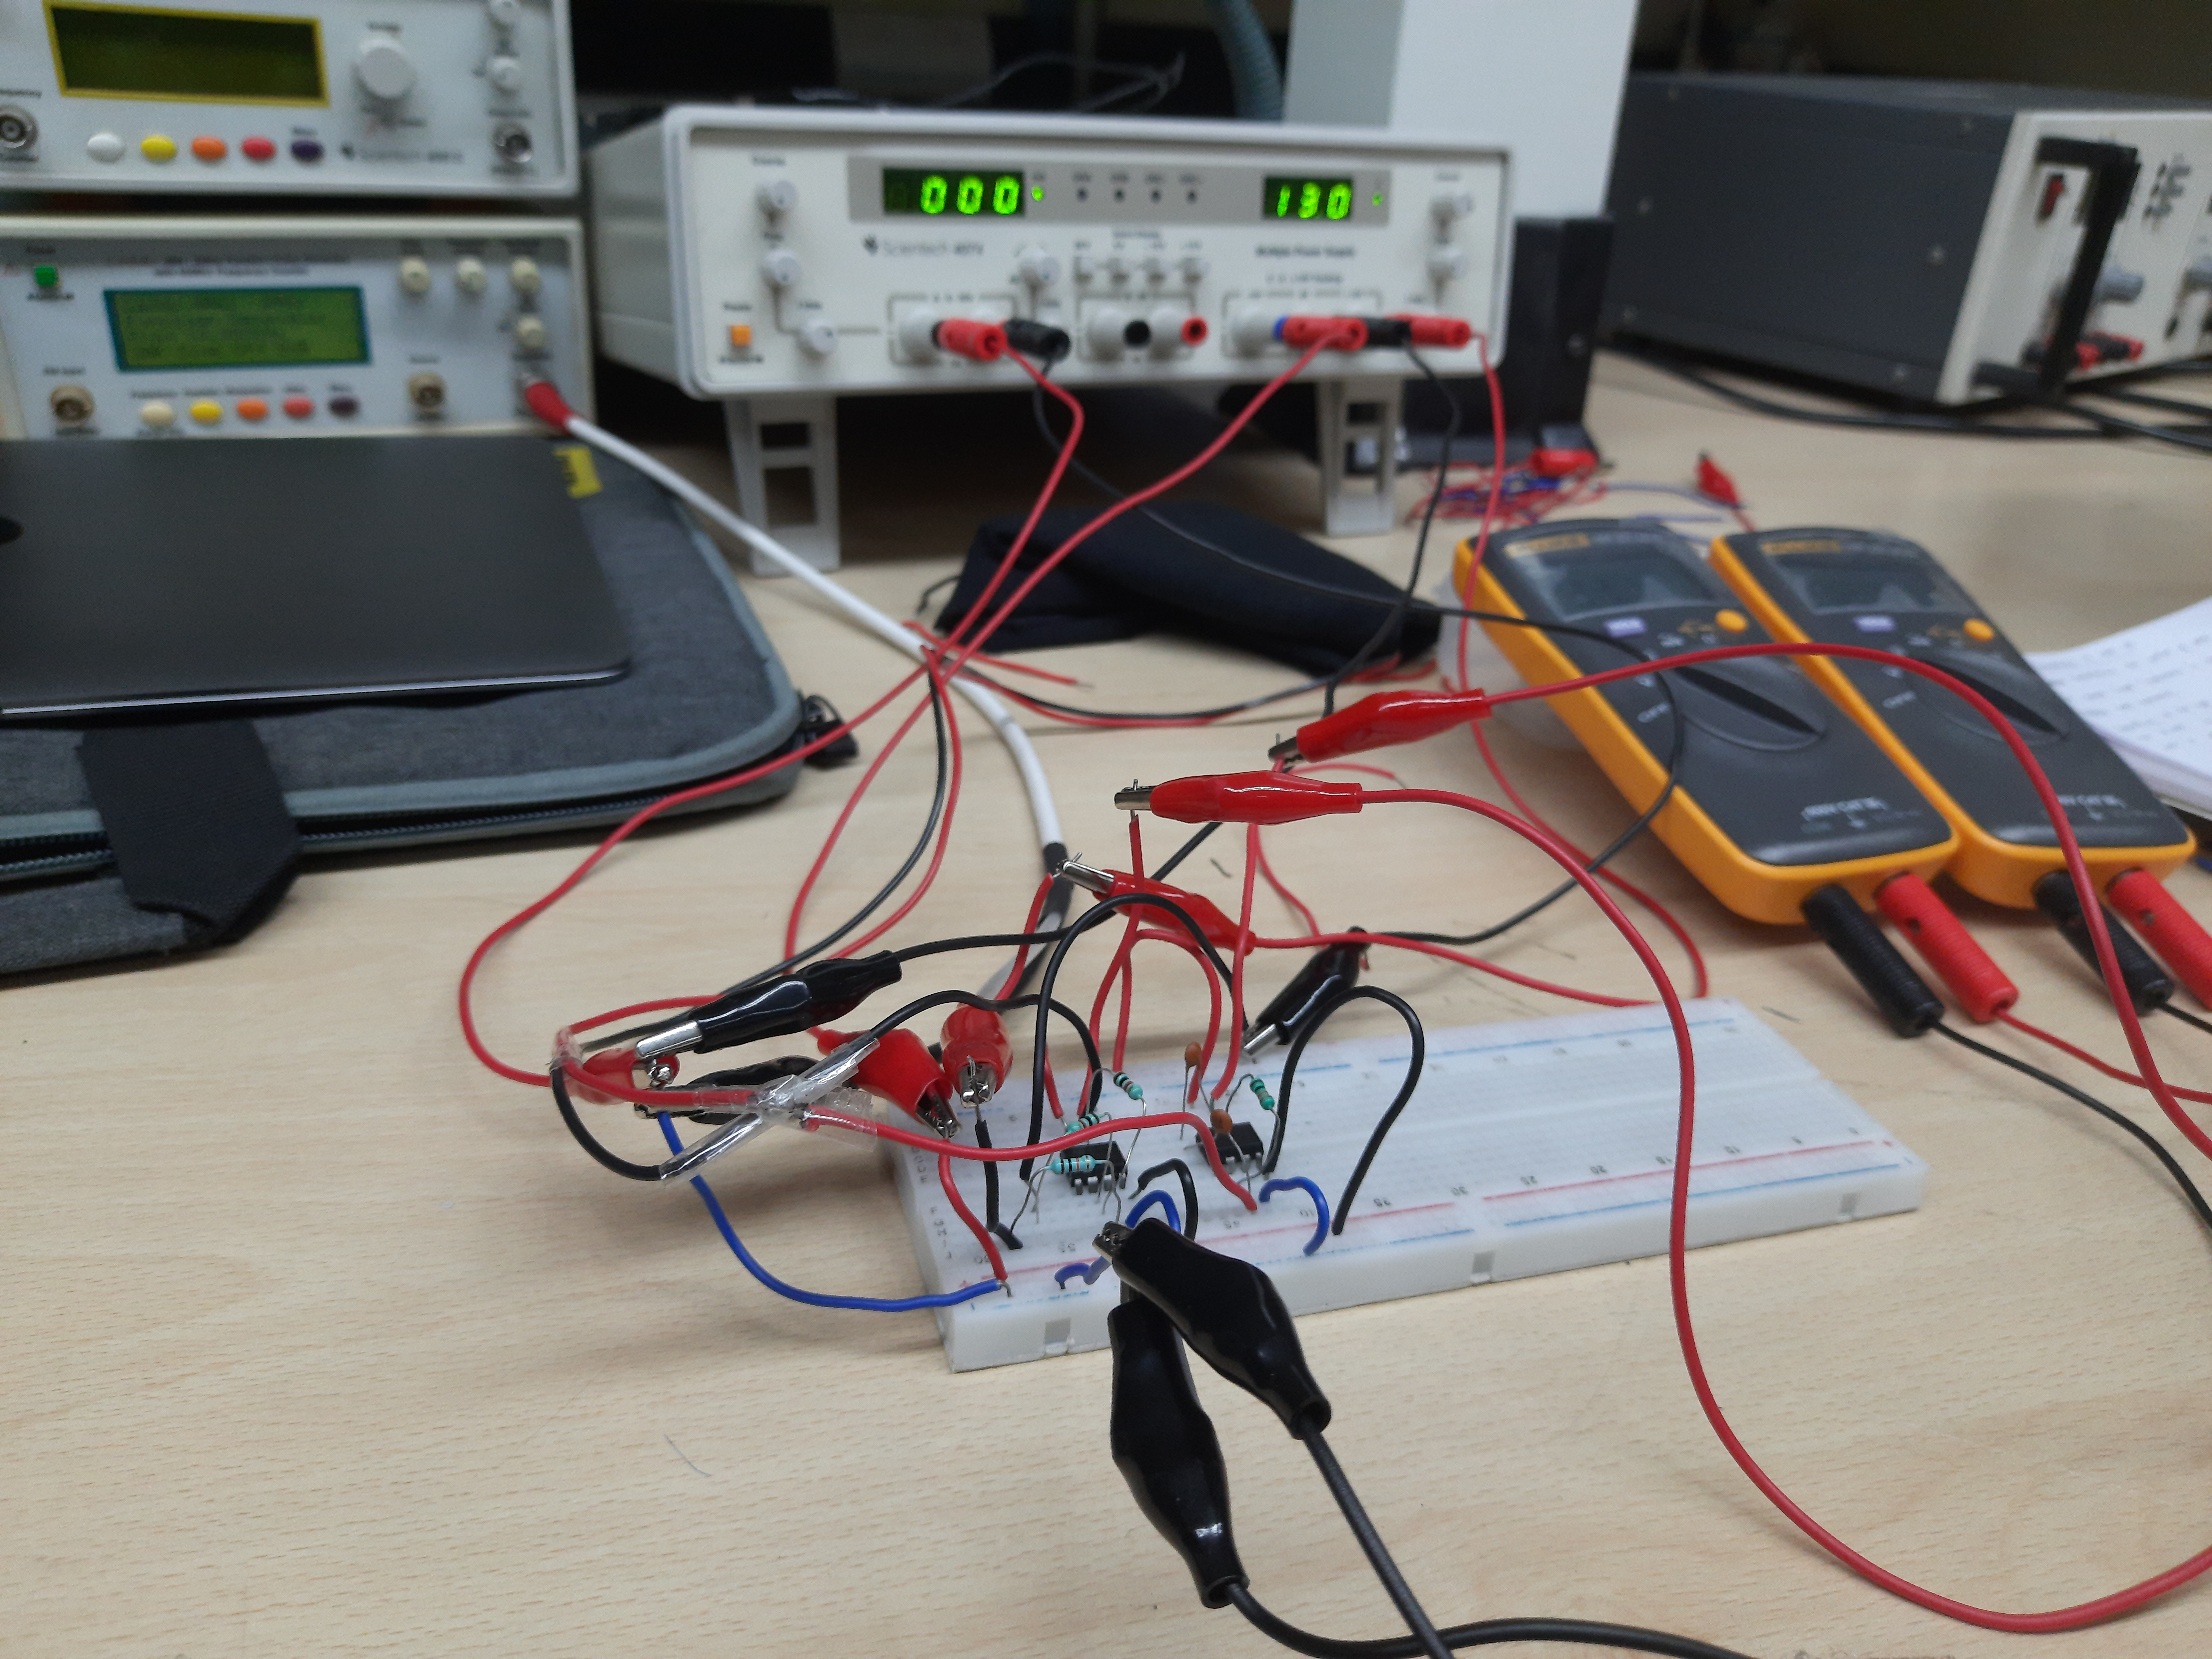
\includegraphics[scale=0.06]{setup}
	\caption{Experimental setup in laboratory}
	\label{s}
\end{figure}

\section{Analysis}
The plot of I-V for Al, Si and Ge at room temperature is as shown in figures (\ref{al}), (\ref{si}) and (\ref{ge}).

\begin{figure}[H]
	\centering
	\includegraphics[scale=0.5]{al}
	\caption{I-V plot for Aluminium at room temperature}
	\label{al}
\end{figure}

\begin{figure}[H]
	\centering
	\includegraphics[scale=0.5]{si}
	\caption{I-V plot for Silicon at room temperature}
	\label{si}
\end{figure}

\begin{figure}[H]
	\centering
	\includegraphics[scale=0.5]{ge}
	\caption{I-V plot for Germanium at room temperature}
	\label{ge}
\end{figure}

It is given that, S=2 mm. Thickness for Al, Si, Ge are 0.16 mm, 0.5 mm and 0.5 mm respectively.
The resistivity of the following materials are calculated as shown below: 

\subsection{Aluminum}
\begin{center}
	S=2 mm\\W= 0.16 mm\\Slope=3.87$\times10^{-4}$ $\Omega$
\end{center}

\begin{equation}
	G_7(W/S)=2Sln(2)/W=17.33
\end{equation}

\begin{equation}
	\rho_o=Slope*(2\pi S)=4.86\times 10^{-7}\Omega m
\end{equation}

\begin{equation}
	\rho=\frac{\rho_o}{G_7(W/S)}=2.80\times10^{-8} \Omega m
\end{equation}

\subsection{Silicon}
\begin{center}
	S=2 mm\\W= 0.5 mm\\Slope=165 $\Omega$
\end{center}

\begin{equation}
	G_7(W/S)=2Sln(2)/W=5.545
\end{equation}

\begin{equation}
	\rho_o=Slope*(2\pi S)=2.07 \Omega m
\end{equation}

\begin{equation}
	\rho=\frac{\rho_o}{G_7(W/S)}=0.37 \Omega m
\end{equation}

\subsection{Germanium}
\begin{center}
	S=2 mm\\W= 0.5 mm\\Slope=7.75$\times10^{-5 }\Omega$
\end{center}

\begin{equation}
	G_7(W/S)=2Sln(2)/W=5.545
\end{equation}

\begin{equation}
	\rho_o=Slope*(2\pi S)=9.7\times10^{-7} \Omega m
\end{equation}

\begin{equation}
	\rho=\frac{\rho_o}{G_7(W/S)}= 1.75\times10^{-7}\Omega m
\end{equation}

To calculate the band gap of Ge, Calculation is as follows:

\begin{table}[H]
	\centering
	\caption{Data for calculation of resistivity and band gap of n-Ge.}
	\label{t1}
	\resizebox{\columnwidth}{!}{%
		\begin{tabular}{|c|c|c|c|c|c|}
			\hline
			\begin{tabular}[c]{@{}c@{}}Temperature \\ ($C^{\circ}$)\end{tabular} &
			\begin{tabular}[c]{@{}c@{}}Temperature \\ (K)\end{tabular} &
			\begin{tabular}[c]{@{}c@{}}Voltage \\ (V)\end{tabular} &
			\begin{tabular}[c]{@{}c@{}}$\rho$\\ $(\Omega m)$\end{tabular} &
			$1/T$ $(1/K)$ &
			$log_e \rho$ \\ \hline
			80  & 353 & 0.15  & 0.06798757772  & 0.00283 & -2.688430271 \\ \hline
			90  & 363 & 0.11  & 0.04985755699  & 0.00275 & -2.998585199 \\ \hline
			100 & 373 & 0.083 & 0.037619793    & 0.00268 & -3.280224957 \\ \hline
			110 & 383 & 0.064 & 0.02900803316  & 0.00261 & -3.540182482 \\ \hline
			120 & 393 & 0.049 & 0.02220927539  & 0.00254 & -3.807245267 \\ \hline
			130 & 403 & 0.037 & 0.01677026917  & 0.00248 & -4.088147653 \\ \hline
			140 & 413 & 0.029 & 0.01314426502  & 0.00242 & -4.331769735 \\ \hline
			150 & 423 & 0.022 & 0.009971511398 & 0.00236 & -4.608023112 \\ \hline
			160 & 433 & 0.018 & 0.008158509326 & 0.00231 & -4.808693807 \\ \hline
			170 & 443 & 0.015 & 0.006798757772 & 0.00226 & -4.991015364 \\ \hline
			180 & 453 & 0.012 & 0.005439006217 & 0.00221 & -5.214158915 \\ \hline
		\end{tabular}%
	}
\end{table}

\begin{figure}[H]
	\centering
	\includegraphics[scale=0.5]{ln}
	\caption{ln($\rho$) versus 1/T plot to determine band-gap of electron.}
	\label{ln}
\end{figure}

\begin{center}
	Slope=4096.19 K\\
	$K$=8.6$\times10^{-5}$ eV/K
\end{center}

Therefore equation (\ref{w}) becomes:
\begin{equation}
	E_g=2.K.slope=0.70 eV
\end{equation}

Error in $E_g$, $\delta E_g=2.K. \delta Slope$=0.06 eV
\newline
\newline
Propagation of error for resistivity, $\rho$ is :
\begin{equation}
	\delta \rho=\rho\left( \sqrt{\left(\frac{ \delta Slope}{Slope}\right)^2+\left(\frac{ \delta W}{W}\right)^2 }\right) 
\end{equation}

\begin{center}
 $\delta \rho_{Al}=0.17\times10^{-8} \Omega m$\\
 $\delta \rho_{Si}=0.008 \Omega m$\\
 $\delta \rho_{Ge}=0.03\times10^{-7} \Omega m$
 
\end{center}


\section{Conclusion}
From this experiment, we found resistivity of Al as $(2.8\pm0.17)\times10^{-8}$ $\Omega m$, resistivity of Si as $0.370\pm0.008$ $\Omega m$, and resistivity of Ge as $(1.75\pm0.03)\times10^{-7}$ $\Omega m$ with the band gap of $0.70\pm0.06$ eV. The literature value of band gap of Ge is 0.68 eV. This implies that this experiment was successful in determining band gap of Ge with percentage errror of 2.94\%. The value of resistivity of Al is as expected, but there have been slight deviation in determining resistivity of Si and Ge since they are semi-conductors, the parameter may depend on various factor such as doping concentration, contact resistance, insulating layers etc may come into picture. Make sure to clean the sample and place the probes in good position to effectively measure the parameter.

\section{References}
\begin{enumerate}
\item{\url{https://www.niser.ac.in/sps/sites/default/files/basic_page/p347_2023/1.Measurement_of_resistivity_and_determination_of_band_gap_using_Four-Probe_method.pdf}}
%\item {\url{}}
\item{\url{https://www.pveducation.org}}


\end{enumerate}

\end{document}